\chapter{Background Research}

This section will start by introducing the client InterDigital, and oneTRANSPORT. This will be followed by a description of the oneM2M standard, including technical details and terminology, as well as the two open source platforms chosen for this project (Eclipse's OM2M and OpenMTC). 

This project involved deploying real sensors connected to an IoT platform, thus will briefly justify the hardware and technology used throughout this project. These include, but are not limited to, Raspberry Pis, Sensor HATs (Hardware Attached on Top), Java, Python, and Digital Ocean's Droplets.

Because the services will be run in different networks, the team will need to address mutual communication capabilities and security concerns. 

Additionally, this report will explain how TLS certificates work in HTTPS, as this was a fundamental feature in development and deployment. It is widely understood that security is very important for the success of IoT \cite{Zhi-KaiZhang2014IoTOpportunities}.

\section{InterDigital}

InterDigital is a research and development company specializing in IoT and wireless technologies for mobiles, services and networks. For their discoveries, they have received tens of thousands of patents. They have a significant presence worldwide, in the United States, Canada, South Korea, Germany, and the United Kingdom \cite{InterDigital2017InterDigitalFACTS}.

In the United Kingdom, InterDigital have adopted the oneM2M standard into their smart transport platform, oneTRANSPORT. At the time of this report, oneTRANSPORT is being trialled in cities round the United Kingdom \cite{InterDigital2016OneTRANSPORT:Today}. Its goal is to demonstrate journey planning, transport event management and incident response applications benefiting from small scale, widespread IoT sensors.

As oneTRANSPORT is being trialled, limited information was provided. It is built using the oneM2M and uses a custom header for authentication and authorization. However, due to the oneM2M standard, this is more than enough knowledge to federate the data from the platform with oneTRANSPORT's server. 

\section{Emergence of Machine to Machine Standards}

OneM2M is a global organisation created with the purpose of standardising Machine to Machine (M2M) communications and IoT technologies. They provide technical specifications in the areas of system architecture, Application Programming Interfaces (API), protocols, reachability / discovery, security solutions, interoperability and more.

These specifications supply a framework for IoT vendors to develop and deploy platforms for services that can be interconnected to the oneM2M environment. By merging the efforts and expertise of worldwide organizations and groups, oneM2M has the capability of facilitating the move to a global interconnected environment.

\subsection{History}

The oneM2M standard was founded in 2012 by eight major SDOs: 

\begin{itemize}
  \item United States: Alliance for Telecommunications Solutions, and Telecommunications Industry Association
  \item Japan: Association of Radio Industries and Businesses, and The Telecommunication Technology Committee
  \item Europe: The European Telecommunications Standards Institute
  \item Korea: Telecommunications Technology Association
  \item China: China Communications Standards Association
  \item India: Telecommunications Standards Development Society India
\end{itemize}

Over time, this standard has significantly grown in popularity. Now, it has more than 200 participating partners including major universities and industry leaders such as Cisco, Intel, and the client, InterDigital.

\subsection{General Architecture}
% References: 5.2.1 functional architecture

OneM2M's functional architecture comprises of a three-layered model, as shown in 5.2.1 \cite{oneM2M2016OneM2MArchitecture}. Here is a list, of descriptions, of them:

\begin{itemize}
  \item \textbf{The Application Layer}\\
  Provides service logic to the system and standard interfaces for managing and interacting with applications. The top layer of the model.
  \item \textbf{The Common Services Layer}\\ Middleware providing functions and services for oneM2M applications such as data management, authorization, authentication and security. This layer also provides a standardized link from application to the underlying network.  
  \item \textbf{The Network Services Layer}\\
  Provides a standardised means for M2M transport and connectivity between different machines. The oneM2M standard abstracts away the specific protocol, allowing implementers to make use of HTTP, CoAP, and more.
\end{itemize}

\begin{figure}[H]
\centering
\makebox[\textwidth][c]{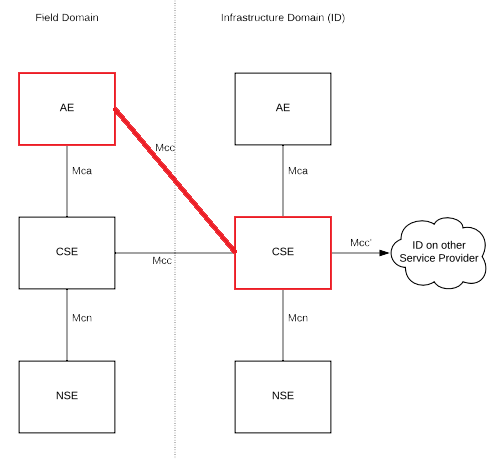
\includegraphics[width=\textwidth]{functional}}
\caption[Functional Architecture]{Functional Architecture taken from oneM2M Functional Architecture \cite{oneM2M2016OneM2MArchitecture}}
\label{fig:fa}
\end{figure}

The basic components in the oneM2M functional architecture diagram, as shown above in figure \ref{fig:fa}, are as follows:

\begin{itemize}
\item \textbf{Application Entity (AE)} \\Part of the application layer that handles the instantiation and management of oneM2M application service logic. Each instance of an AE is given a unique AE-ID. Communications from or to AE are done through Mca reference points (reference points are explained in section \ref{sec:rp}). 

An example of an AE developed in this project is the camera streaming application. It takes images from the Raspberry Pi camera and pushes them across the Mcc reference point shown in figure \ref{fig:fa}. This is highlighted in red.

\item \textbf{Common Services Entity (CSE)} \\Part the common services layer that handle the instantiation of a set of common core functions and services such as data management, device registration and security. These are exposed to other entities through reference points (Mca, Mcc, Mcn). CSEs are allocated unique CSE-IDs.    

\item \textbf{Network Services Entity (NSE)} \\Part of the network service layer providing services from the underlying network to the CSE. To simplify the architecture, NSE components and communication (Mcn reference point) will be overlooked. To view the full architecture, see oneM2M Functional Architecture \cite{oneM2M2016OneM2MArchitecture}.   
\end{itemize}

\subsection{Reference points}
\label{sec:rp}
% References: 5.2.2 functional architecture

The reference points mentioned in the functional architecture (Mca, Mcc, Mcc' and Mcn) are defined as communication flows between entities. They are distinguished between the entities. The "Mc-" structure is shorthand for M2M communication 5.2.2 \cite{oneM2M2016OneM2MArchitecture}. 

\begin{itemize}
  \item \textbf{Mca}\\ 
  Communications between AE and CSE. Gives the AE the ability to use services from the CSE. 
  \item \textbf{Mcc}\\ 
  Communications between two CSEs. Gives CSEs to use services by other CSEs.
  \item \textbf{Mcc'}\\ 
  Communications between two infrastructure domains (ID). Two CSE's (both Infrastructure Nodes) that reside in different service provider domains. 
\end{itemize}

\subsection{OneM2M nodes}
% References: 6.1 functional architecture

Nodes are logical entities that are identifiable with the oneM2M system and can either be CSE or Non-CSE capable 6.1 \cite{oneM2M2016OneM2MArchitecture}. 

\begin{figure}[H]
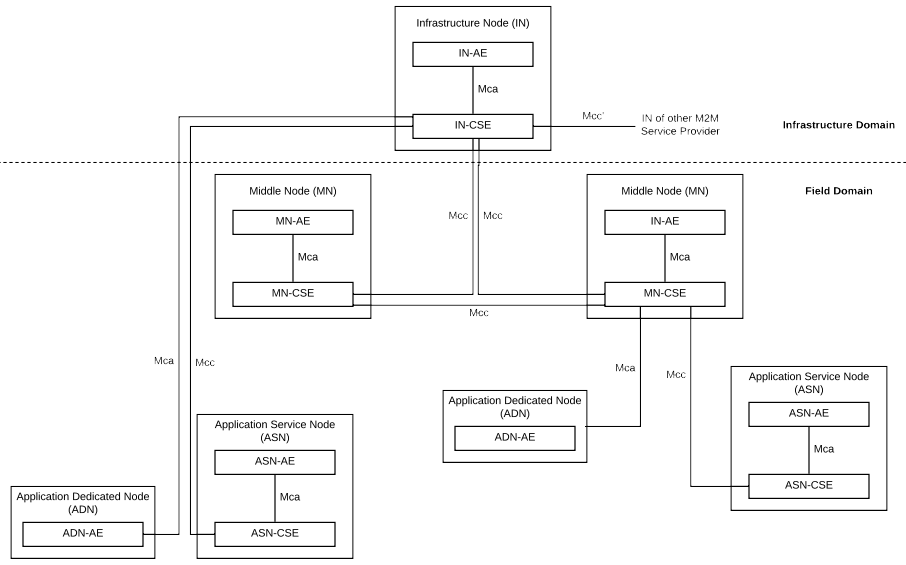
\includegraphics[width=\textwidth]{nodes}
\caption[Supported configuration of oneM2M with reference point communications taken from oneM2M Functional Architecture]{Supported configuration of oneM2M with reference point communications taken from oneM2M Functional Architecture \cite{oneM2M2016OneM2MArchitecture}}
\label{fig:nodes}
\end{figure}

Figure \ref{fig:nodes} demonstrates the possible combinations of oneM2M nodes with communications between nodes shown as reference points (Mca, mcc and mcn). Figure \ref{fig:nodes} has overlooked Mcn reference points and Non-oneM2M nodes. OneM2M supports the following nodes with their corresponding characteristics \cite{oneM2M2016OneM2MArchitecture}:

\begin{itemize}
  \item \textbf{Infrastructure Node (IN)}\\ 
  Contains one CSE and zero or more AEs. Only one IN in the infrastructure domain of a oneM2M service provider. CSEs in INs may contain functions that are unique. 
  \item \textbf{Middle Node (MN)}\\ 
  Contains one CSE and zero or more AEs. CSEs in MNs may contain functions that are unique. 
  \item \textbf{Application Server Node (ASN)}\\ 
  Contains one CSE and one or more AEs. CSEs in ASNs may contain functions that are unique. An ASN is also a leaf node.
  \item \textbf{Application Dedicated Node (ADN)}\\ 
  Contains no CSEs and one or more AEs. An ADN is also a leaf node.
\end{itemize}

Domain types \cite{oneM2M2016OneM2MArchitecture}:

\begin{itemize}
  \item \textbf{Infrastructure Domain}\\ 
  In the context of a M2M service provider, contains only one infrastructure node.
  \item \textbf{Domain field}\\ 
  Contains zero or more ASNs, ADNs and MNs of a M2M service provider.
\end{itemize}

The general architecture of an oneM2M environment consists of one infrastructure node (IN-CSE) connected to one or more MN-CSEs. MNs and INs contain AEs which implement the application logic; they acquire and process data.

Leaf nodes containing AEs can be implemented with ASN or ADN and are registered to MNs or INs. The main difference between leaf nodes and the other nodes is the ability to be registered to. ASNs and ADNs are leaf nodes, therefore they cannot be registered to. MNs are intermediate nodes and INs are root nodes. This project will only look at MNs and INs.  

\subsection{API Service Layer Core Protocol Specification}

OM2M architecture is resource-based and the entire system is exposed to an interoperable RESTful API \cite{oneM2M2016OneM2Mservicelayer} over all the reference points (mca, mcn, mcn and mcc'). 

Request/Response primitives are represented in either XML or JSON formats. The process of translating primitives into XML or JSON is called serialization. The act of serialization is performed when transmitting primitives over communication protocols (HTTP, CoAP, MQTT). 

\subsection{Communication Protocols Specification}

OneM2M's overall system requirements specifies that the system shall allow multiple communication methods based on IP access that accommodates for constrained and rich computing (processing and memory) and communications (2/3/4G, wireless, wired) \cite{oneM2M2016OneM2Mservicelayer}.

Therefore, oneM2M has specifications for the following communications protocols on the application layer of the TCP/IP model:

\begin{itemize}
  \item HTTP (HyperText Transfer Protocol) \cite{oneM2M2016OneM2MBindingb}: The communications protocol for the world wide web. Flexible, with massive support but ultimately too cumbersome for certain constrained Internet of Things communications.
  \item MQTT (MQ Telemetry Transport) \cite{oneM2M2016OneM2MBinding}: A flexible, binary pipe designed specifically for constrained Internet of Things communications.
  \item CoAP (Constrained Application Protocol) \cite{oneM2M2015OneM2MBinding}: A protocol designed both for interoperability with the web, as well as for constrained Internet of Things communications.
\end{itemize}

For this project, HTTP was the sole communication protocol used as deploying a platform in constrained environments are not in the requirements of the client. Future work could, and likely should involve investigating the differences between MQTT and CoAP, and how to apply them. 

\subsection{Communication within M2M Service Provider}
% Reference: 6.4 functional architecture

CSE enabled nodes would perform the operation of registration with other CSE nodes. This enables a CSE to use functions of another CSE. AEs shall register to CSE enabled nodes to be able to use functions and communication offered by that CSE 6.4 \cite{oneM2M2016OneM2MArchitecture}. Table \ref{onem2m-communication-procedures} demonstrates the supported CSE and AE registrations as well as the procedure.  

\begin{table}[H]
\centering
\begin{tabular}{|l|l|l|}
\hline
\textbf{Originator} & \textbf{Receiver(s)} & \textbf{Procedure}               \\ \hline
MN-CSE              & IN-CSE, MN-CSE       & CSE registration                 \\ \hline
MN-AE               & MN-CSE               & \multirow{2}{*}{AE registration} \\ \cline{1-2}
IN-AE               & IN-CSE               &                                  \\\hline
\end{tabular}
\caption{oneM2M Communication Procedures}
\label{onem2m-communication-procedures}
\end{table}

The registration procedures of the AE listed in table \ref{onem2m-communication-procedures} will not be explained in this report but are explicitly explained in oneM2M functional Architecture specification \cite{oneM2M2016OneM2MArchitecture}. CSE registration procedure is explained in the implementation section \ref{sec:federation}.  

\subsection{Communication inter M2M Service Provider}
% Reference: 6.5 functional Architecture

This project is focused on federating data in platforms from  different service providers. OneM2M functional specification \cite{oneM2M2016OneM2MArchitecture} have specified how this communication should occur. The reference point \lstinline{Mcc'} is responsible for inter platform communication which has the following characteristics:\\ 

\begin{itemize}
  \item IN-CSEs are the access points of both M2M domains. All inter communication  attempts go through the root IN before reaching AEs in middle (MNs) or leaf nodes (ASNs, ADNs). 
  \item IN-CSE need to be on public IPs for mutual communication.
\end{itemize}


\subsection{OneM2M Resources}

Entities (Data, AEs, CSEs, etc.) inside the oneM2M system are represented as resources organised in a resource tree, a structure built for representing a group of resources. They follow the follow principles:

\begin{itemize}
	\item All resources have a none editable resource type (from a pre-defined list) used for resource identification
\end{itemize}

Below is a list and description all the resource types used in this project, for a complete list of resource types, please see the oneM2M specification. 

\begin{itemize}
  \item \textbf{Type 1: AccessControlPolicy}\\ Access control rules for defining which entities can perform which operations. It is the underlying decision access logic.
  \item \textbf{Type 2: ApplicationEntity}\\Contains information about the Application Entity when registered to a CSE. 
  \item \textbf{Type 3: Container}\\Represents a container for container instances. The maximum number of instances can be specified, creating a rolling database. If the maximum number of instances is 10, then when an 11th content instances gets added, the oldest content instance will be removed. 
  \item \textbf{Type 4: ContentInstance}\\Data instances such as sensor values, images, etc.
  \item \textbf{Type 5: CSEBase}\\Represents the CSE and is the root the resource tree hierarchy.
  \item \textbf{Type 16: RemoteCSE}\\Represent a  remote CSE that is registered to the current CSE. This resource while a direct child of the registered CSEBase. Navigable. 
\end{itemize}   

\subsection{OneM2M Open Source Implementations}

There exist multiple platforms implemented using the oneM2M standard. The oneM2M website contains a list of known open source implementations \cite{oneM2M.org2017OneM2MProjects}.

\begin{itemize}
  \item \textbf{KETI OCEAN \cite{KETI2018OCEAN}}\\
  While initially promising, it requires registration to acquire source code, and licensing is unclear. Additionally, of the little documentation that exists, it typically is either in Chinese or is poorly translated.
  \item \textbf{OpenDayLight IOTDM \cite{OpenDayLightIoTDMProject}}\\
  Seemingly abandoned, with no clear source code or binaries to download. It has possibly been forgotten or abandoned.
  \item \textbf{Eclipse OM2M \cite{EclipseFoundation2015EclipseCommunication}}\\
  Developed by Eclipse in France using Java, well maintained (recent version released on the 21 of October 2017). Forum and bug trackers and active community. 
  \item \textbf{ATIS oneM2M}\\
  To download, or even view the documentation, requires the user to apply to participate in ATIS oneM2M. As participation is only granted to "member-based organisations (such as ATIS)", governmental agencies, or those who will actively contribute.
  \item \textbf{IoT OASIS SI \cite{iotoasis2017Iotoasis/SIIntegration}}\\
  Of the little documentation that exists, virtually all of it is in Korean. None of the team can read Korean, and the lack of English documentation proves that the software is immature, and hence unsuitable for this project.
  \item \textbf{OpenMTC \cite{OpenMTC2017OpenMTC}}\\
  Released to Open source 7th of November 2017 with recent updates. Written in Python. Active community that responds well to issues.
\end{itemize}

After reviewing the pros and cons of each open source platform, the team decided to deploy the OM2M platform with an AE for gathering sensor data. This would then show interoperability with InterDigital's oneTRANSPORT IN-CSE.

Halfway through the project, the team discovered OpenMTC's recent release \cite{OpenMTC2017OpenMTC}, and so decided to show both interoperability between two open source platforms, in addition to oneTRANSPORT.

\section{Eclipse OM2M}

Eclipse OM2M is an open source Java implementation of the oneM2M standard. It is built using the Java Open Services Gateway initiative standard making extensive use of plug-ins. To connect the sensors, a new plug-in that communicates with the sensors in response to user interaction or subscriptions would need to be created. OM2M developer’s documentation \cite{om2mdeveloper} was used to install the dependencies for plug-in development. 

OM2M has example light plug-in used for controlling virtual lights through the OM2M platform \cite{Eclipse2018OM2M/one/WebEclipsepedia}. This was used as a guide for the plug-in interacting with sensors from the Raspberry Pi.

\subsection{Light Plug-in}
\label{light plugin}

The plug-in implemented on the OM2M platform was modelled after the sample plug-in, used for controlling lights, under the name \lstinline{org.eclipse.om2m.ipe.sample}. The sample plug-in had many features which could be altered to fit required needs. Following the instructions on the Eclipse OM2M developer page \cite{om2mdeveloper} the plug-in was instantiated with the proper settings and configuration.

\begin{figure}[H]
  \centering
  \frame{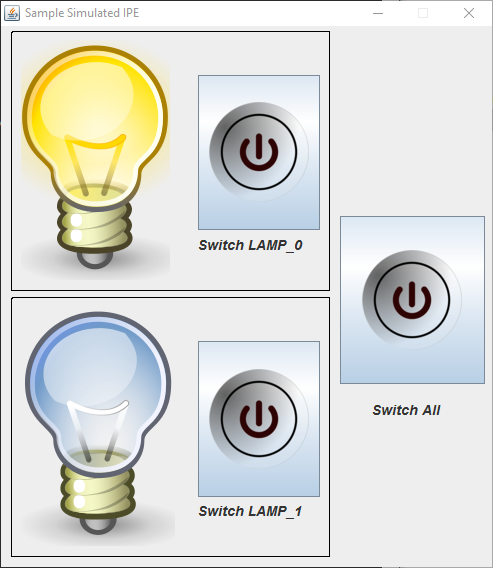
\includegraphics[width=0.5\textwidth]{lamps}}
  \caption{OM2M Sample Simulated IPE}
  \label{fig:sample-simulated-ipe}
\end{figure}

Figure \ref{fig:sample-simulated-ipe} shows the graphical user interface (GUI) of the virtual light controls run on the MN-CSE gateway. The MN-CSE will be directly connected to the IoT lights. The user can switch the lights on or off by interacting with the GUI in figure \ref{fig:sample-simulated-ipe}, or by interacting with the registered IN-CSEs RESTful API.\\

\begin{lstlisting}[caption={Interacting with lights using REST}, label={lst:lights}]
POST https://sensivision.co/~/in-cse-id/in-name/mn-cse-id/mn-name/LAMP_0?op=setOn&lamp_id=LAMP_0
POST https://sensivision.co/~/in-cse-id/in-name/mn-cse-id/mn-name/LAMP_0?op=setOff&lamp_id=LAMP_0
\end{lstlisting}

The REST calls mentioned above would be sent to the IN-CSE and are used for turning \lstinline{LAMP_0} on and then off. The lights can be controlled remotely through the REST API. This assumes that the MN-CSE, which has a unique ID \lstinline{mn-cse-id} and name \lstinline{mn-name}, is registered to the IN-CSE with the unique ID \lstinline{in-cse-id} and name \lstinline{in-name}.

The resource structure inside the IN-CSE will be:\\

\dirtree{%
.1 \lstinline{BaseCSE(IN)}. 
.2 \lstinline{RemoteCSE(MN)}. 
}
\clearpage
While the resource structure inside the MN-CSE will look like:\\

% Use this instead of ascii art. the number denotes depth.
\dirtree{%
.1 \lstinline{BaseCSE(MN)}. 
.2 \lstinline{RemoteCSE(IN)}. 
.2 \lstinline{Application Entity (LAMP\_0)}. 
.3 \lstinline{Container (DESCRIPTION)}. 
.4 \lstinline{One Content Instance containing REST calls for lamp 0}.
.3 \lstinline{Container (DATA)}. 
.4 \lstinline{Content Instances for each REST call (contains data about the lamp's state, lampId, location and type)}.
.2 \lstinline{Application Entity (LAMP\_1)}. 
.3 \lstinline{Container (DESCRIPTION)}. 
.4 \lstinline{One Content Instance containing REST calls for lamp 1}.
.3 \lstinline{Container (DATA)}. 
.4 \lstinline{Content Instances for each REST call (contains data about the lamp's state, lampId, location and type)}.
.2 \lstinline{Application Entity (LAMP\_ALL)}. 
.3 \lstinline{Container (DESCRIPTION)}. 
.4 \lstinline{One Content Instances containing REST calls for all lamps}. 
}

CSE functions on the IN can interact with the CSEs that are registered to it. Specifically, the MN contains functionality and logic (AE) for interacting with a virtual light. the final visualization can be seen in figure \ref{light} and enables the IN to have light controlling function by forwarding message to the MN-CSE. 

\begin{figure}[H]
  \centering
  \frame{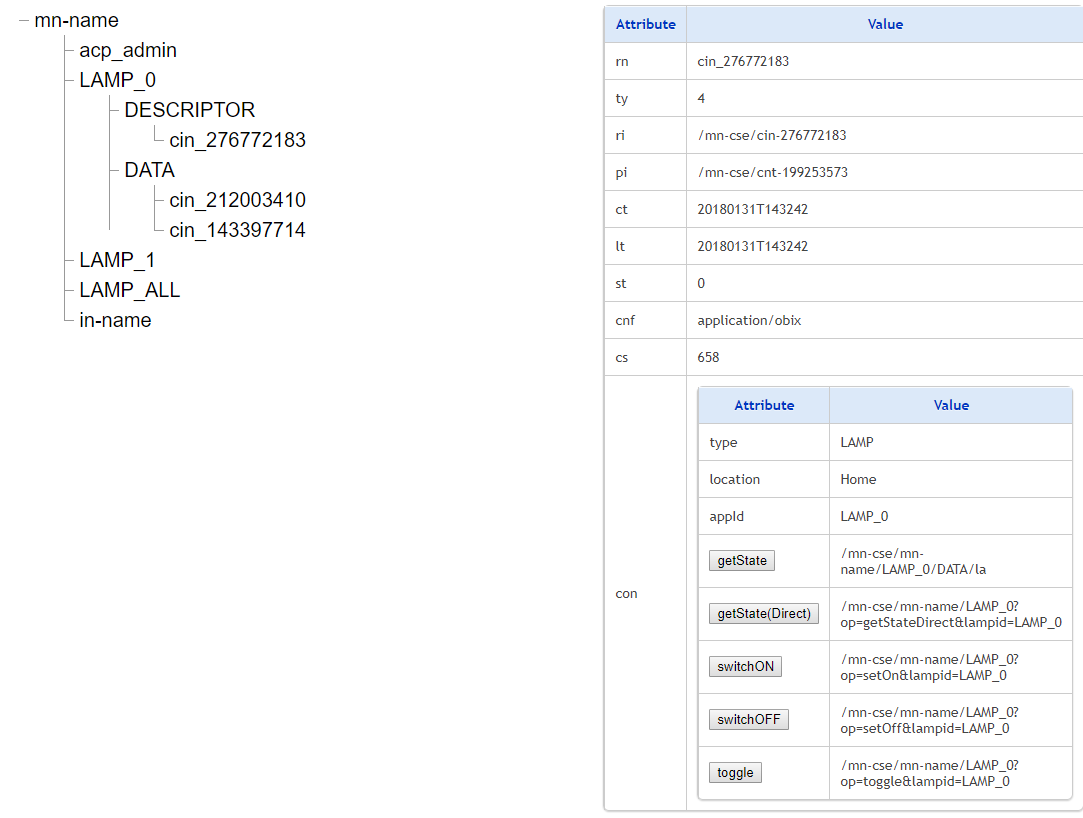
\includegraphics[width=\textwidth]{lamp}}
  \caption{Visual Interaction with IN for light controls}
  \label{light}
\end{figure}

Although this plug-in has many features that were used to build the plug-in for interacting with the Raspberry Pi sensors, it did not implement remote data storage (storage on the IN instead of the MN).

\section{OpenMTC}

OpenMTC\cite{OpenMTC2017OpenMTC} is an open source implementation of the oneM2M standard written in python. It was publicly released on November 7th, 2017 on Github. OpenMTC's approach is to simplify the integration with other devices. It uses specific terminology:

\begin{itemize}
  \item \textbf{Backend}: oneM2M IN-CSE.
  \item \textbf{Gateway}: oneM2M MN-CSE.
\end{itemize}

Because this project was already using Python scripts for gathering the data, it was decided to add an extra task of duplicating the sensor interaction application on OpenMTC to compare  and contrast different publicly available platforms. This as easy because all the Python scripts could simply be run by OpenMTC, in a similar manner to OM2M. Additionally, the Python scripts could be integrated into the OpenMTC plug-in, avoiding the forking overhead.

\section{Existing Work}

OneM2M have a specification on interoperability \cite{oneM2M2016OneM2Minter} and organize a yearly international conference for platform federation testing. The documentation specifies example requests and response syntax over HTTP, CoAP and MQTT for industry platforms to test whether their solution conforms to the oneM2M standard.

\section{Hardware}

From the oneM2M architecture, the MN-CSEs would act as gateways between IN-CSEs hosted on the cloud and sensor devices. Their functionality is solely for collecting data when necessary and pushing it to the IN for storage. Therefore, they do not need to be powerful machines. In a real-world environment these devices would be small so in the end, micro controllers were used due to their size and hardware capabilities. On the other hand, the INs would be responsible for storing the data and federating it, this would require a far more high specification machine that is publicly accessible. 

\subsection{Development Boards}

A development platform was needed to build the project. For an IoT platform a small, low powered board is generally considered desirable. Due to the time pressures of this project, it was important that the board be readily available, with plenty of documentation, so easy to develop for. Due to this, using a typical laptop or desktop was immediently discounted, opting to look at microcomputers instead. There are innumerable microcomputers available nowadays with widely varying capabilities. The team evaluated different platforms to decide which was best

\begin{table}[ht]
\begin{tabularx}{\textwidth}{|l|X|}
\hline
\textbf{Platform} & \textbf{Notes} \\
\hline
Laptop & Powerful and easy to use, but large and difficult to attach sensors to as no modern laptop has any form of GPIO. AS a result, to connect sensors either USB breakout boards, or the microphone jack would have to be used. This is far from ideal.\\
\hline
Arduino & Widely popular and with massive open source support. However, the boards themselves are typically lacking in horsepower and would be unable to run networked Python or Java. Video streaming would be out of the question. \\ 
\hline
Raspberry Pi & A cheap and popular microcomputer that can run a full Linux distribution with massive popularity. Additionally, some of the team have experience working with Raspberry Pis.\\ 
\hline
Intel Edison & Compared to Arduino and Raspberry Pi, the platform while powerful enjoys little attention. This is hardly surprising considering that the platform is in the process of being discontinued \cite{2017ProductAction}. \\ 
\hline
 & Other devices were considered but ultimately ignored due to factors including, but not limited to poor market share, bad documentation, and / or low performance.\\ 
\hline
\end{tabularx}
\caption{Evaluating Different Platforms}
\label{evaluating-differernt-platforms}
\end{table}

Ultimately it was decided that a Raspberry Pi would be the best choice.

\subsection{Raspberry Pi}

The Raspberry Pi is a handy credit-card sized microcomputer with a moderately powerful ARM System-on-Chip solution, and plenty of I/O (USB, Ethernet, WiFI, Bluetooth, HDMI, GPIO, i2c, CSI, DSI, etc.) - perfect for the project. As a bonus, the team each all had received Raspberry Pis a couple years prior, so some of the team were familiar with the board.  

\subsection{Accessories}

After deciding to use a Raspberry Pi, accessories were needed: microSD card, USB power supply, a method of writing disk images, and an internet connection. The first three were provided by InterDigital, and the last is provided by instructing the Raspberry Pi to automatically connect to the universities open WiFi network whenever possible. Now, with the Raspberry Pi configured, booting, and ready to develop for, all the team needed to do was demonstrate the protocol using an interesting data source.

\subsection{GPIO Sensors}

It was decided that it would be interesting and useful to connect sensors measuring the environment up to oneM2M, as it closely mirrors InterDigital's activities with their oneTRANSPORT platform. The question now, is what sort of sensors were wanted, and how to connect them to the Raspberry Pi?

Initially, the team investigated purchasing a bundle of individual sensors, break out cables, and breadboards from an internet retailer. Approaching the problem like this would result in a completely customisable and configurable platform that would be easy to extend in future. After all, while the group is entirely composed of computer scientists, the team experience with breadboards and hardware due to Computer Systems II.

However, while attaching sensors directly, or indirectly to the GPIO headers certainly has its advantages, it comes with its own set of disadvantages. Connecting individual sensors while extensible is fragile. By choosing individual sensors whenever the group, or the client decided to transport and setup the platform in a new location, or even pack it away for the day, every sensor would need to be carefully connected back up using the correct ports. This would have been a time consuming and error prone process.

So, while attaching real-world sensors to the board was a good idea, using individual sensors was not the right approach.

\subsection{Hardware Attached on Top}

Investigating further, it was discovered that the Raspberry Pi foundation has created a specification for Hardware Attached on Top. These HATs are typically a single board with a GPIO header that connects directly to the Raspberry Pi. The idea being that instead of every accessory manufacturer connecting independently and incompatibly, a common form factor and communications protocol (Over i2c) is decided. This allows different accessories to slot directly into the Raspberry Pi and work together. As a bonus, many of these HATs can be found for sale from speciality online retailers.

After comparing the different HATs, the Raspberry Pi Sense HAT, shown in figure \ref{fig:pi} was chosen as it provided essentially everything required in an easy to use, reliable and robust form factor. This handy module slots into the Raspberry PI's GPIO (General Purpose Input / Output) header, with screw holes around the edge to securely connect it to the board.

The Sense HAT provides an $8\times8$ LED matrix, joystick and the following sensors:

\begin{itemize}
  \item Accelerometer (Movement sensor)
  \item Barometer (Pressure sensor)
  \item Hygrometer (Humidity sensor)
  \item Magnetometer (Compass)
  \item Thermometer (Temperature sensor)
  \item Three Axis Gyroscope (Rotation sensor)
\end{itemize}

\begin{figure}[H]
  \centering
  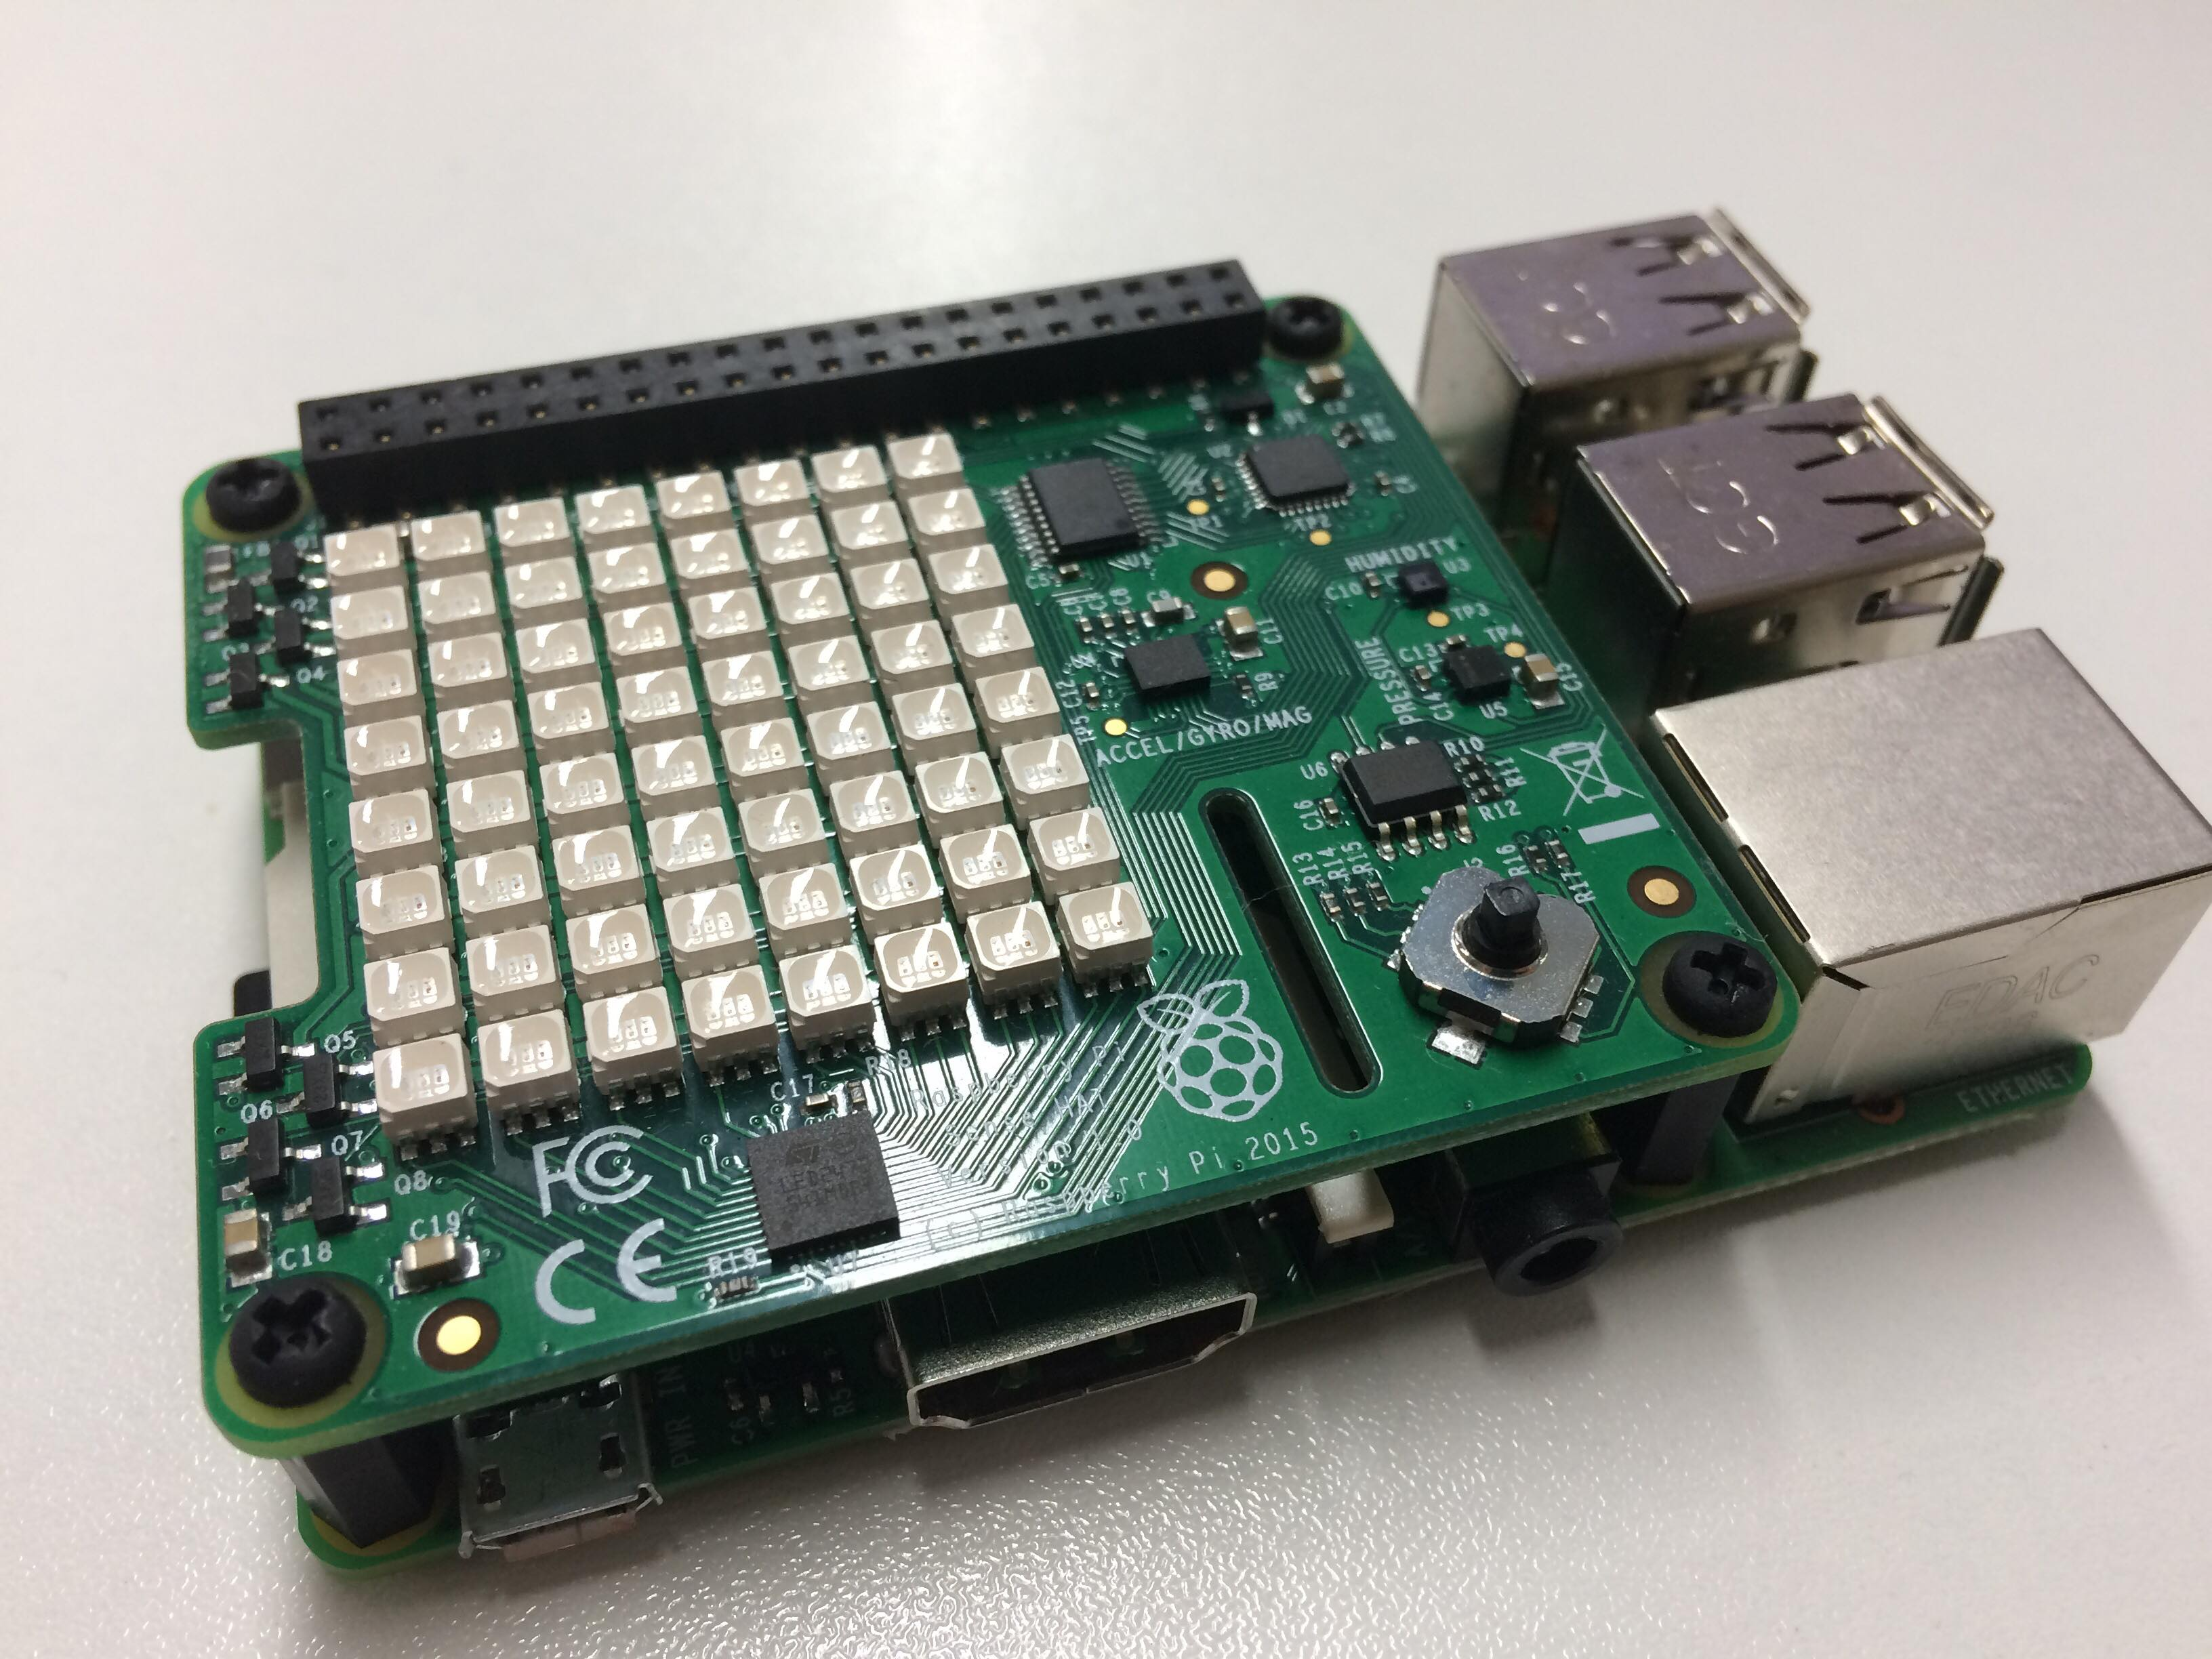
\includegraphics[width=\textwidth]{pi}
  \caption[Raspberry Pi with Sense HAT]{Raspberry Pi with Sense HAT}
  \label{fig:pi}
\end{figure}

Additionally, other values can be read directly from the Raspberry Pi itself such as time, WiFi signal strength, processor load, memory usage, and more. This is more than enough for simple uses, and the $8\times8$ LED matrix (It can be seen in figure \ref{fig:pi}) allows visual feedback to the user to help them use the product. With financial backing and approval from InterDigital, two were purchased.

To the use the Sense HAT, the user has the choice of manually sending i2c commands and toggling GPIO pins or using a very handy python library named \lstinline{sense-hat} \cite{RaspberryPiFoundation2017SenseHAT} which comes pre-installed with Raspbian-lite. To save time, the latter option was chosen.

\subsection{Camera}

\begin{figure}[H]
  \centering
  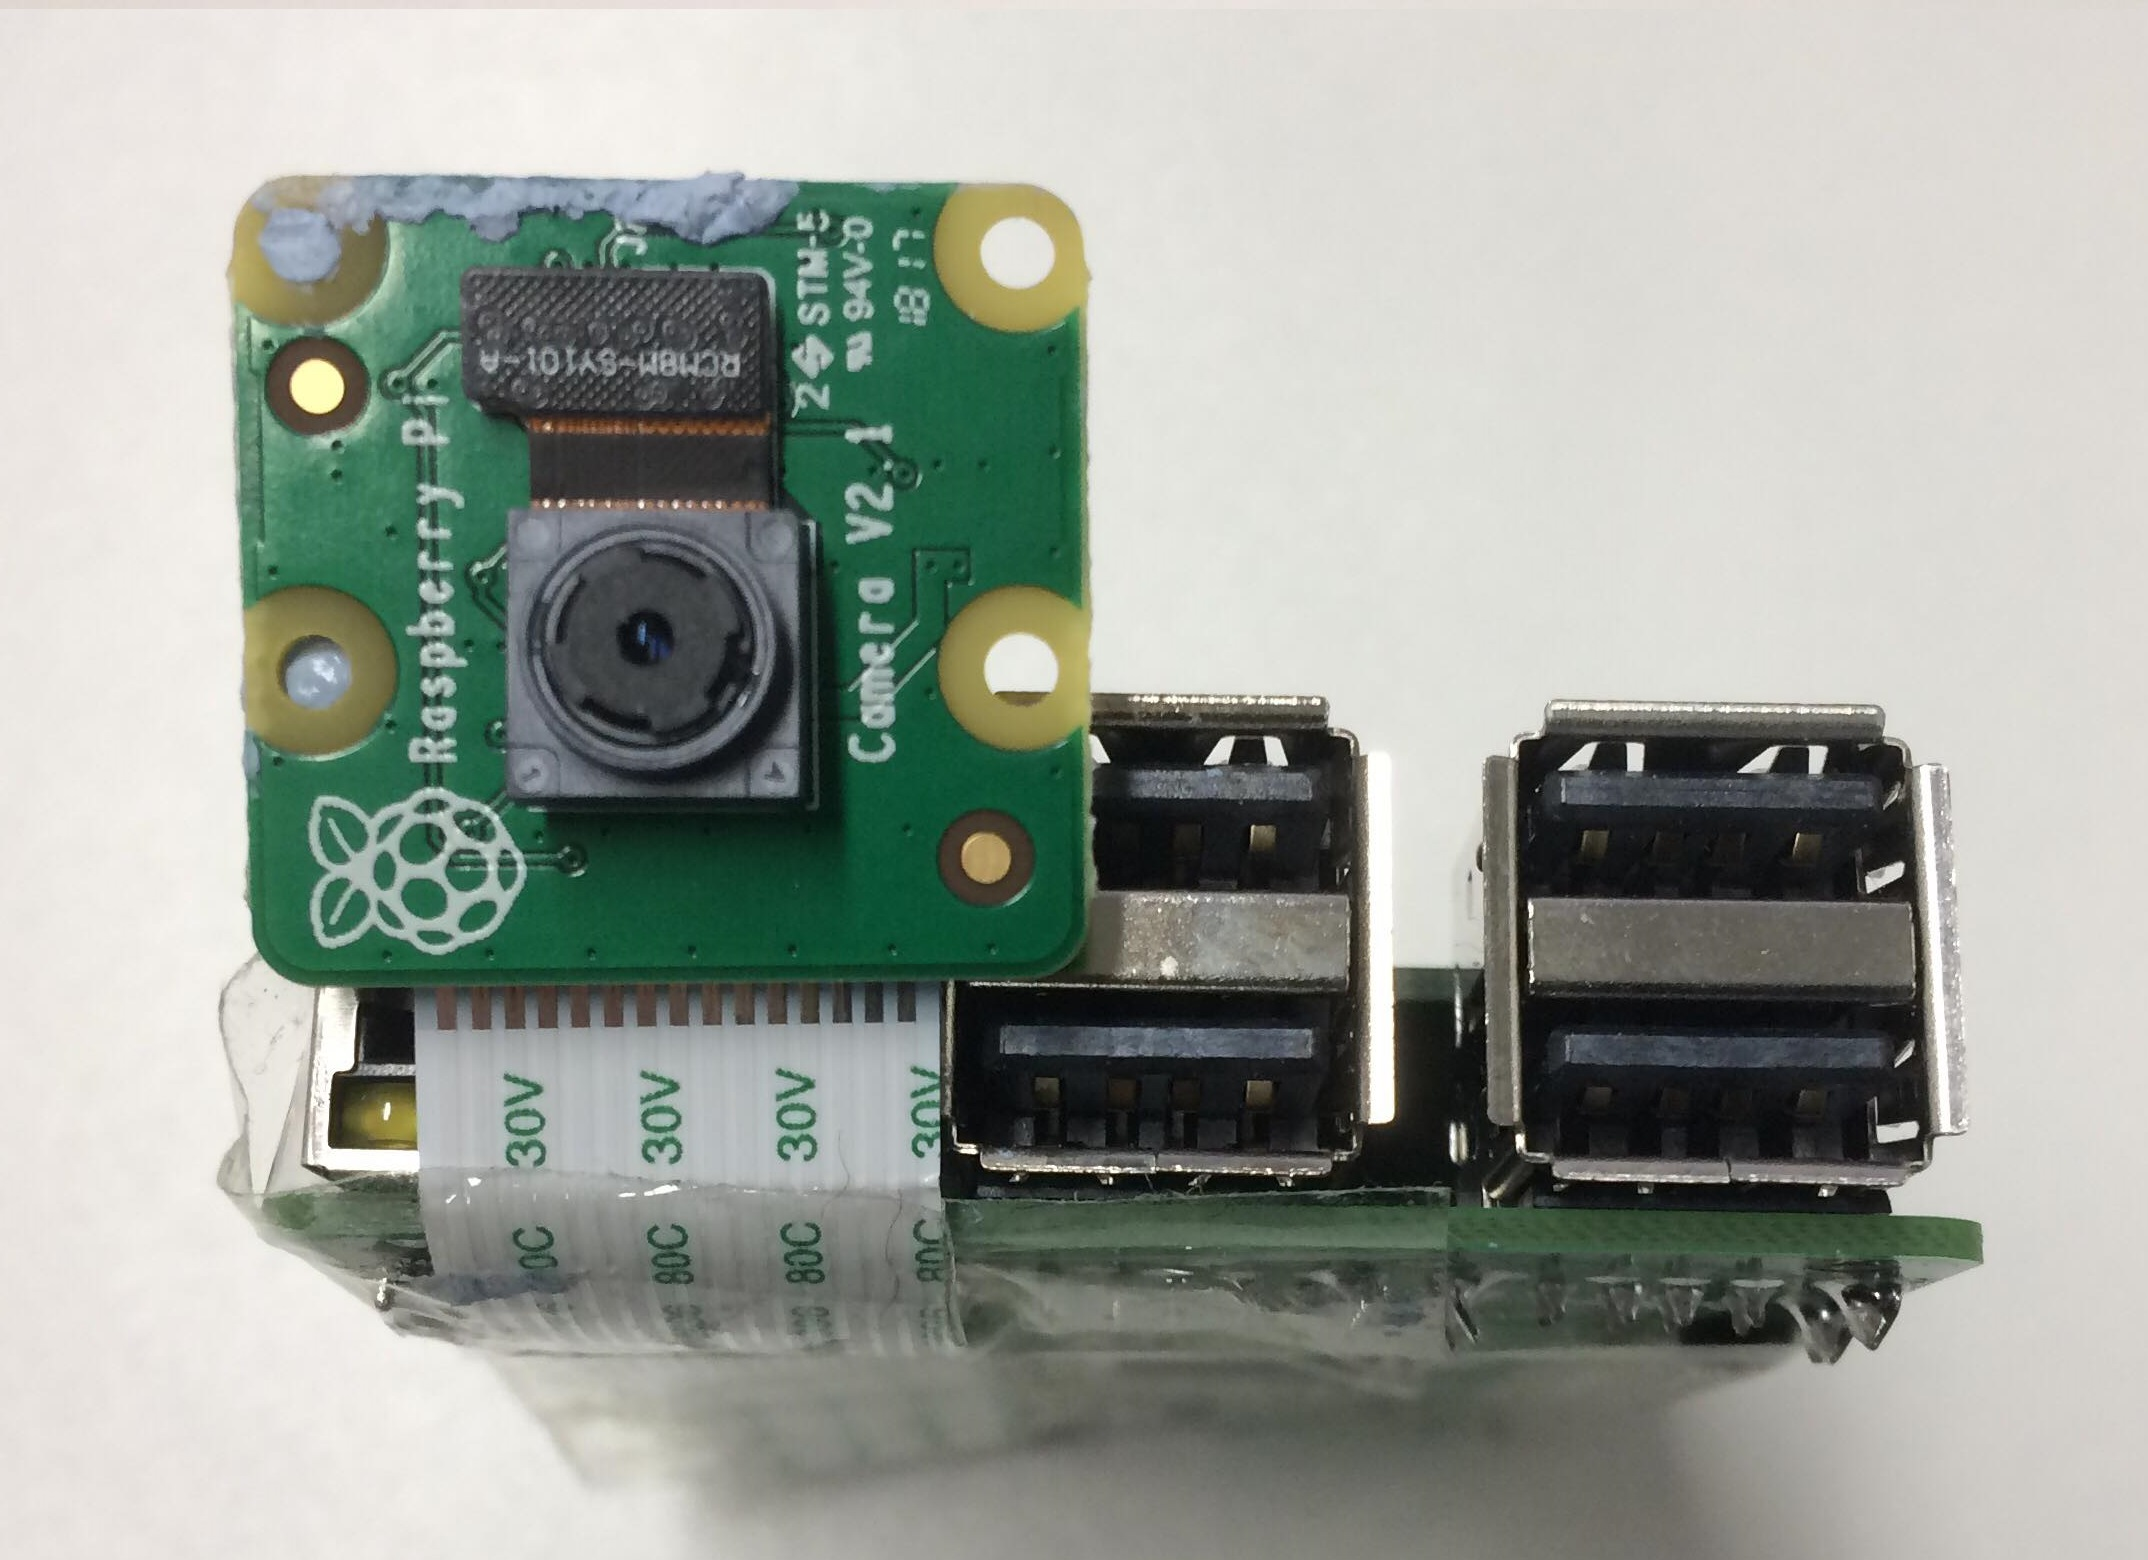
\includegraphics[width=\textwidth]{camera}
  \caption[Raspberry Pi with camera]{Raspberry Pi with camera}
  \label{fig:camera}
\end{figure}

However, as time passed it was determined that the Sense HAT sensors were not enough. InterDigital were interested in investigating video streaming through oneM2M. In addition to passing single values the team wanted to pass large and complicated data streams, showing the limits of the standard and platform.

In addition to the GPIO header, the Raspberry Pi contains a serial, camera header that allows the user to connect a camera to the device using a flat-flex ribbon cable. As the flex-flex ribbon cable was rather long, it was wrapped around the device, and secured with sticky tape and blue tack.

Research shows that in 2013, Michael Kirwan, of the Continua Health Alliance had at the very least discussed and intended to attempt to stream video over oneM2M \cite{MichaelKirwan2013VideoNetwork.}. This finding proved that oneM2M was likely capable of streaming video, even if the resolution of 528$\times$324 at 14 frames per second was poor. Now, the question was, how could the team recreate such a set-up, using OM2M?

After purchasing and installing a Raspberry Pi Camera V2.1 (can be seen in figure \ref{fig:camera}), it was tested using \lstinline{raspistill -o /tmp/test.jpg}, and \lstinline{raspivid -o /dev/null}, confirming that everything was working. The next step would be to integrate it with oneM2M. 

\subsection{Cloud Service}

To federate an open source platform with oneTRANSPORT, the IN-CSE had to be hosted a routable public IP address. Originally, the team was using InterDitial's Cloud platform provider (Azure), but after running into some configuration issues that would significantly halt the progress of the project, this was moved to another server. 

University Virtual Machines \cite{UniversityofSouthampton2017VMService} were deemed unsuitable for this project as full control of the virtual machine was deemed necessary. Plus, unlike commercial offerings, the university has significant lag times when it comes to provisioning new virtual machines and is reluctant to open them up to the wider internet.

GitHub Education package offers \$50 credit towards Digital Ocean droplet servers \cite{Github2018StudentPack}. As members of team had experience in configuration for droplet servers it was decided to use DigitalOcean droplet as the cloud hosted IN.

However, because of oneM2M MN-CSE architecture, there would be routing issue when the web hosted IN communicates with the MN which sits inside a network using Network Address Translation (NAT). 

\section{Routability Issue}

OneM2M's gateways (MN-CSEs) and servers (IN-CSEs) both run web servers and use HTTP(S) to communicate between each other. 

\begin{figure}[H]
  \centering
  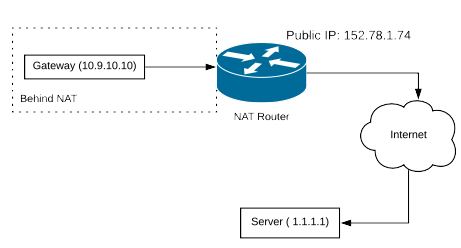
\includegraphics[width=\textwidth]{nat}
  \caption[NAT outgoing traffic]{NAT outgoing traffic}
  \label{fig:net}
\end{figure}

In this environment (see figure \ref{fig:net}), the gateway is located on a network behind NAT (Network Address Translation) resulting in the server not being too able to directly communicate with the gateway. From the server in figure \ref{fig:net}, the private IP address \lstinline{10.9.0.0/24} is not routable from outside the NAT network. 
  
The overall goal of NAT is make up for the lack of IPv4 public addresses with the use of private addresses (typically \lstinline{192.168.0.0/24}, or \lstinline{10.9.0.0/24}). Outgoing traffic will be routed correctly. The NAT router will be responsible for translating outgoing traffic to use the public IP address and make sure that the response is routed to the correct IP inside the NAT network. Clients / server model with request response functions properly with the NAT router using dynamic port forwarding. 
    
The problem comes trying to establish a connection from IN-CSE to the MN-CSE. The NAT router will receive the request from the In-CSE but will not know what private IP to forward it to inside the NAT network, as the gateway as not sent out any communications. 

The team investigated two solutions to resolve this problem, using VPNs (OpenVPN) and using SSH port forwarding.  

\subsection{Virtual Private Network (VPN)}

A virtual private network (VPN) is a used to create a secure and encrypted network connection over a less secure network. VPNs operate on the transport layer of the TCP/IP model. VPN was mainly developed to enable remote clients to securely access corporate applications and other resources.

\subsection{SSH Port Forwarding}

SSH (secure shell) is a protocol for accessing one computer from another though an encrypted tunnel. There are many applications of SSH including transferring files and running commands, but SSH will be used to establish a virtual private network between the IN-CSE and the NATed MN-CSE. SSH operates on the application level of TCP/IP.\\

\begin{lstlisting}[caption={SSH port forwarding}, label={lst:ssh1}]
ssh -R sourcePort:forwardToHost:onPort connectToHost
\end{lstlisting}

The command from the listing \ref{lst:ssh1}, when run on the host, will attempt to connect (through SSH) to \lstinline{connectToHost} and forward all connection attempts to \lstinline{localhost:sourcePort} on the remote host to \lstinline{forwardToHost:onPort} on the host.

In the context of oneM2M, the MN-CSE will be running behind NAT on port \lstinline{8181}. It would tell the IN-CSE that the PoA of the MN-CSE is \lstinline{localhost:8181} and run this command on the MN-CSE setting up a SSH tunnel to the IN-CSE:\\

\begin{lstlisting}[caption={SSH port fowarding with Values}, label={lst:ssh2}]
ssh -R 8181:localhost:8181 IN-CSE
\end{lstlisting}

When the IN-CSE receives a connection attempt to localhost:8181, it would forward it through the SSH tunnel to the MN-CSE on port 8181. The MN-CSE is now directly accessible from the IN-CSE. 

\subsection{Solution}

Because of its simplicity and easy configuration, VPNs were used between the MN-CSEs and IN-CSE to achieve mutual accessibility. OpenVPN \cite{OpenVPN2018OpenVPNVPN} is a widely used open source VPN for establishing secure connections between Internet components.

In addition to bypassing to NAT, a VPN adds an extra layer of security to MN-CSE IN-CSE communications. Encrypting data such that even HTTP will be protected against attackers. Although this provides additional security between MN and IN, the plain text protocol HTTP is used by default for accessing IN data. This would be a security concern as messages could be intercepted and tampered with.    

\section{Security, TLS Certificates and HTTPS}

The secure version of HTTP, HTTPS, uses key exchange protocols to establish a secure symmetric key for encrypting and decrypting traffic. One of the methods for key exchanging without a Man in the Middle gaining knowledge of the symmetric key uses asymmetric cryptography, also known as public key / private key cryptography. 

HTTPS uses Certificate Authorities to verify server certificate came from the correct server. This allows clients to authenticate servers they have never visited previously. Unlike protocols such as SSH and GPG, every device or application that implements HTTPS maintains a central Certificate Store. This store defines a list of root CAs that are trusted above all others, and form the start of the chain of trust.

As a side note, VPNs such as OpenVPN just like SSH and GPG do not have a central Certificate Store and instead depend on the user distributing certificates. This has the added benefit that a rouge CA cannot create a fake certificate for your VPN, and they are never involved in the first place. 

The team encountered problems with certificates, so knowledge of how TLS certificates work in HTTPS is essential. They are built with asymmetric cryptography (public / private keypairs), Hashes (MD5, SHA-256), digital signatures and CAs. 

When a client initially connects to a web server, it needs to verify the server claims to be who he says. The server will respond to the client with its certificate. The certificate consists of:

\begin{itemize}
  \item Domain name
  \item Expiry date
  \item Public key of the server
  \item Other Details
\end{itemize}

The hash of the certificate is also sent encrypted with the server’s private key that it only knows. This is a form of digital signature from the server as it is the only one that can encrypt the hash the content to maintain the integrity of the certificate being sent over an insecure network. But an attacker can operate a Man In The Middle Attack by acting as the server by generating his own public/private key pair and replacing certificate with his own as well as the public key and encrypted hashed content with his private key. How will the client verify this? 
 
CAs verify and sign the whole certificate of a domain by encrypting it with their private key and distributing the associated public key to web browsers for verification. In the case mentioned above where an attacker would perform a MITMA by injecting his own certificate and public/private key pair, this would not be signed by a CA and therefore a browser would raise a warning mentioning that the connection may not be secure.

There is an optional step where the server would perform client verification like the steps mentioned above. Applied to oneM2M, HTTPS connection require a valid TLS certificate. LetsEncrypt was chosen as the CA to sign a valid certificate for sensivision.co due to the free, automated certificate verification and generation process.

\clearpage
